\chapter{Tutorial 1: creating a Matrix class available in Excel}


As I have mentioned before, \xlp has a generic way to handle container. In this tutorial we will look at this method and will create a matrix class than can be directly handled by \xlp. 


\section{A class Matrix}


Below the definition of a Matrix class compatible with \xlp.

\

\begin{verbatim}
class Matrix:
 
	def __init__(self, rows, cols):
 		self.rows = rows
 		self.cols = cols
  	self.datas = range(self.rows*self.cols)

 	def __len__(self): 
  	return len(self.datas)

 	def __setitem__(self, index, value):
  	self.datas.__setitem__(index, value)

 	def __getitem__(self, index):
  	return self.datas.__getitem__(index)
 
 	def size1(self):
  	return self.rows
  	
  def size2(self):
  	return self.cols
  	
\end{verbatim}

\

You can see that we need to define the methods \_\_len\_\_, \_\_setitem\_\_,  \_\_getitem\_\_, size1 and size2.

\

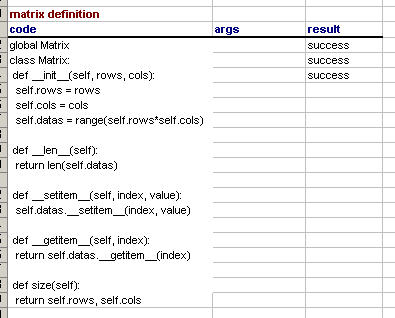
\includegraphics[width=12cm]{images/matrix1.jpg}


\section{Matrix creation}

To create the matrix, we need to generate an empty matrix with correct dimensions "\_Matrix(\_rows, \_cols)" and fill it with the values arguments. 

\ 

Here the result:

\

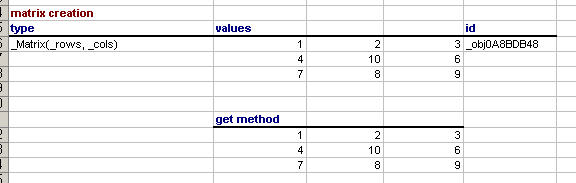
\includegraphics[width=12cm]{images/matrix2.jpg}
